%\documentclass{beamer}
%\documentclass[c]{beamer}
 \documentclass[t]{beamer}
%\documentclass[b]{beamer}
\listfiles

\mode<presentation>
{
 \usetheme[english]{KIT}
% \usetheme[usefoot]{KIT}
%   \usetheme[deutsch]{KIT}

%%  \usefonttheme{structurebold}

  \setbeamercovered{transparent}

  %\setbeamertemplate{enumerate items}[circle]
  \setbeamertemplate{enumerate items}[ball]
}

\usepackage{babel}
\date{\today}
%\DateText

%\KITfoot{\parbox[t]{90mm}{\today:\qquad Dies ist eine sehr lange selbstdefinierte Fu\ss{}zeile -- Dies ist eine sehr lange selbstdefinierte Fu\ss{}zeile -- Dies ist eine sehr lange selbstdefinierte Fu\ss{}zeile}}


\usepackage[latin1]{inputenc}
\usepackage[TS1,T1]{fontenc}
\usepackage{array}
\usepackage{lipsum}
\newcommand{\KeY}{Ke\kern-0.1emY}
\usenavigationsymbols
%\usenavigationsymbols[sfHhdb]
%\usenavigationsymbols[sfhHb]

\title{Seamless Interactive Program Verification\\ Demo of AlgoVer}

\author{Sarah Grebing, Mattias Ulbrich, Jonas Klamroth}
\subtitle{\insertauthor{}}
\institute{Institut f�r Theoretische Informatik, KIT}

\KITtitleimage[width=\titleimagewd]{../../Bilder/screenshotpres2018.png}





\begin{document}

\begin{frame}
  \titlepage
\end{frame}

\begin{frame}{Interactive Program Verification}

\only<1> { 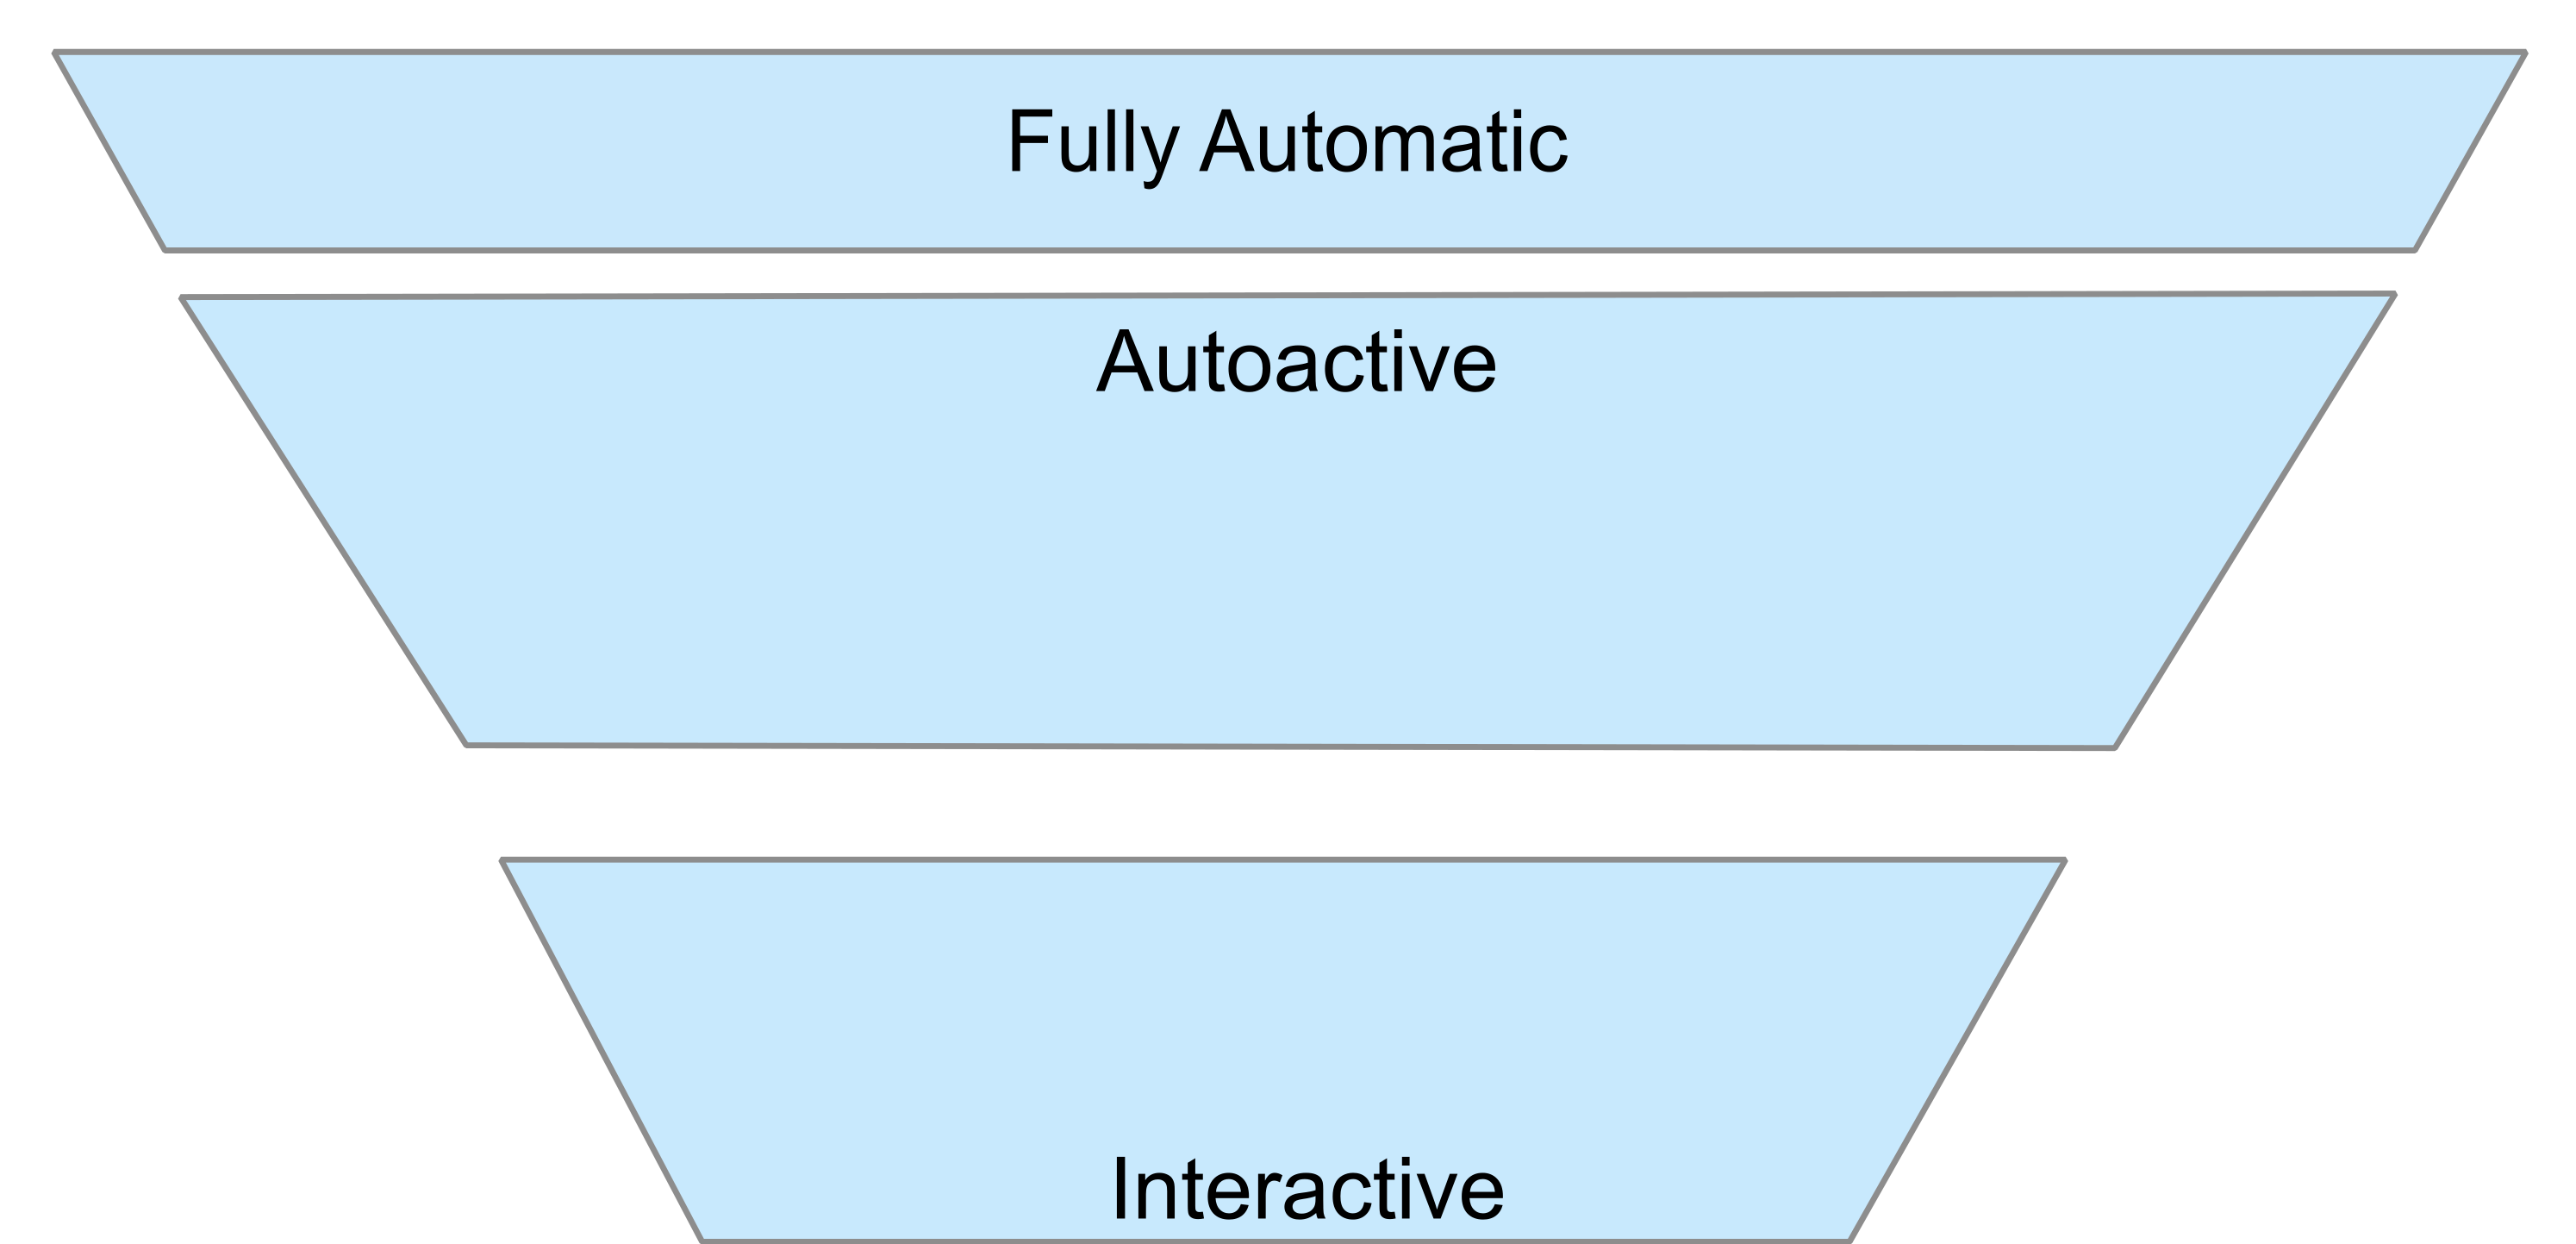
\includegraphics[width=\textwidth]{ipv1.png}}
\only<2> { 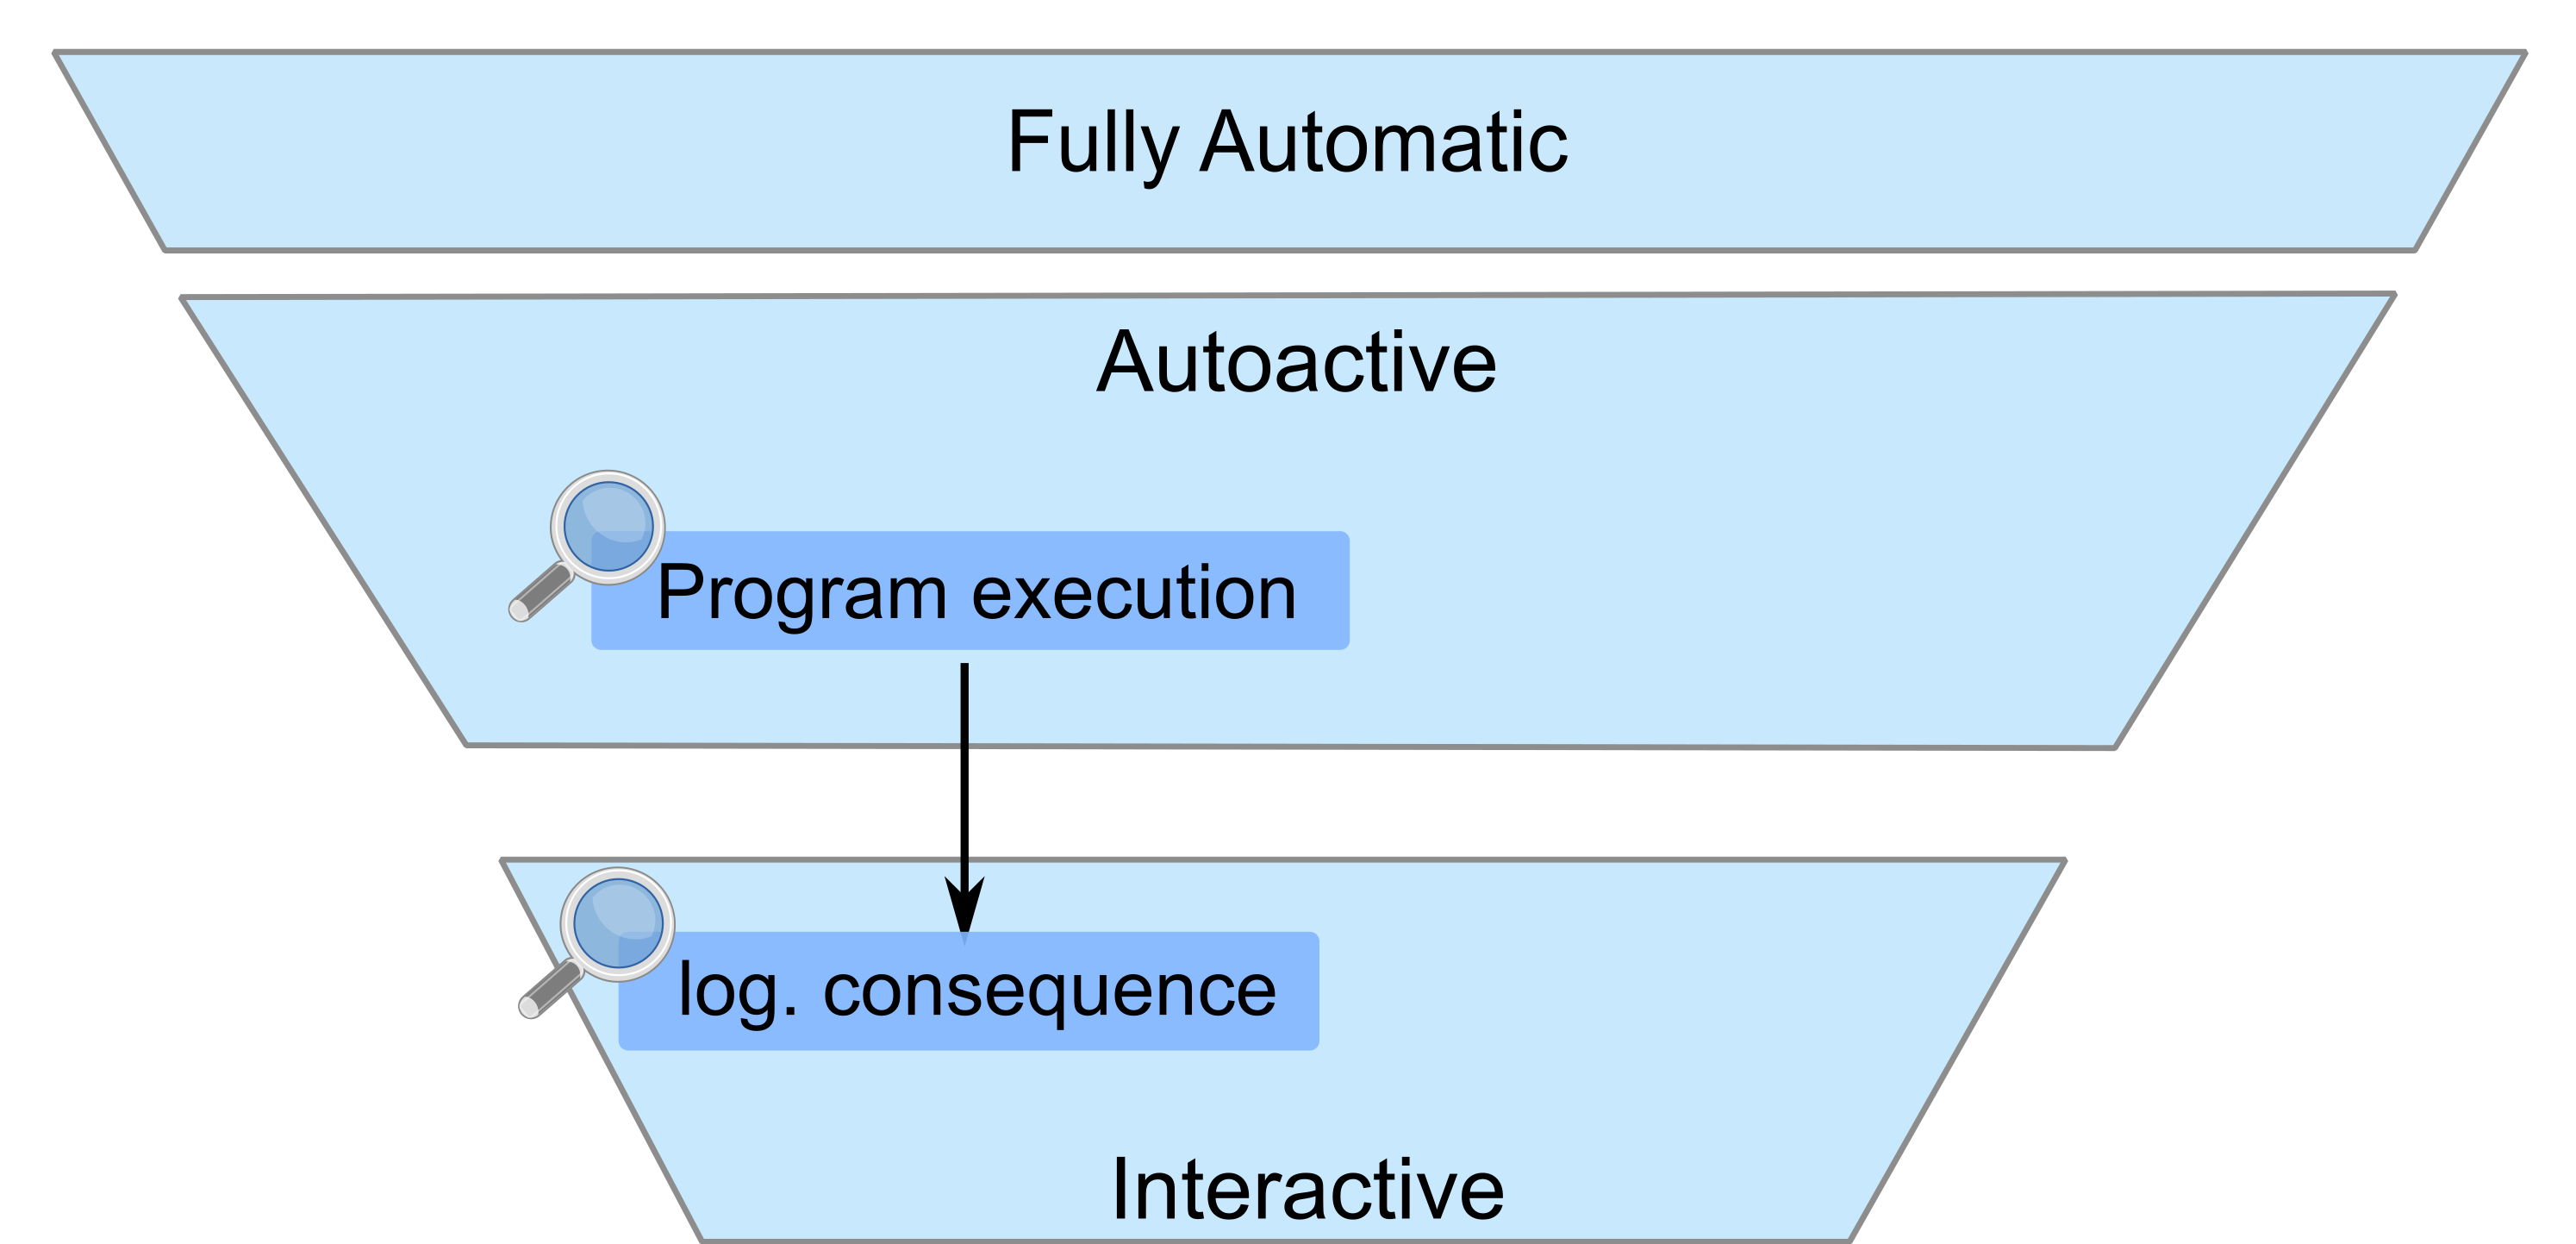
\includegraphics[width=\textwidth]{ipv2.png}}
\only<3> { 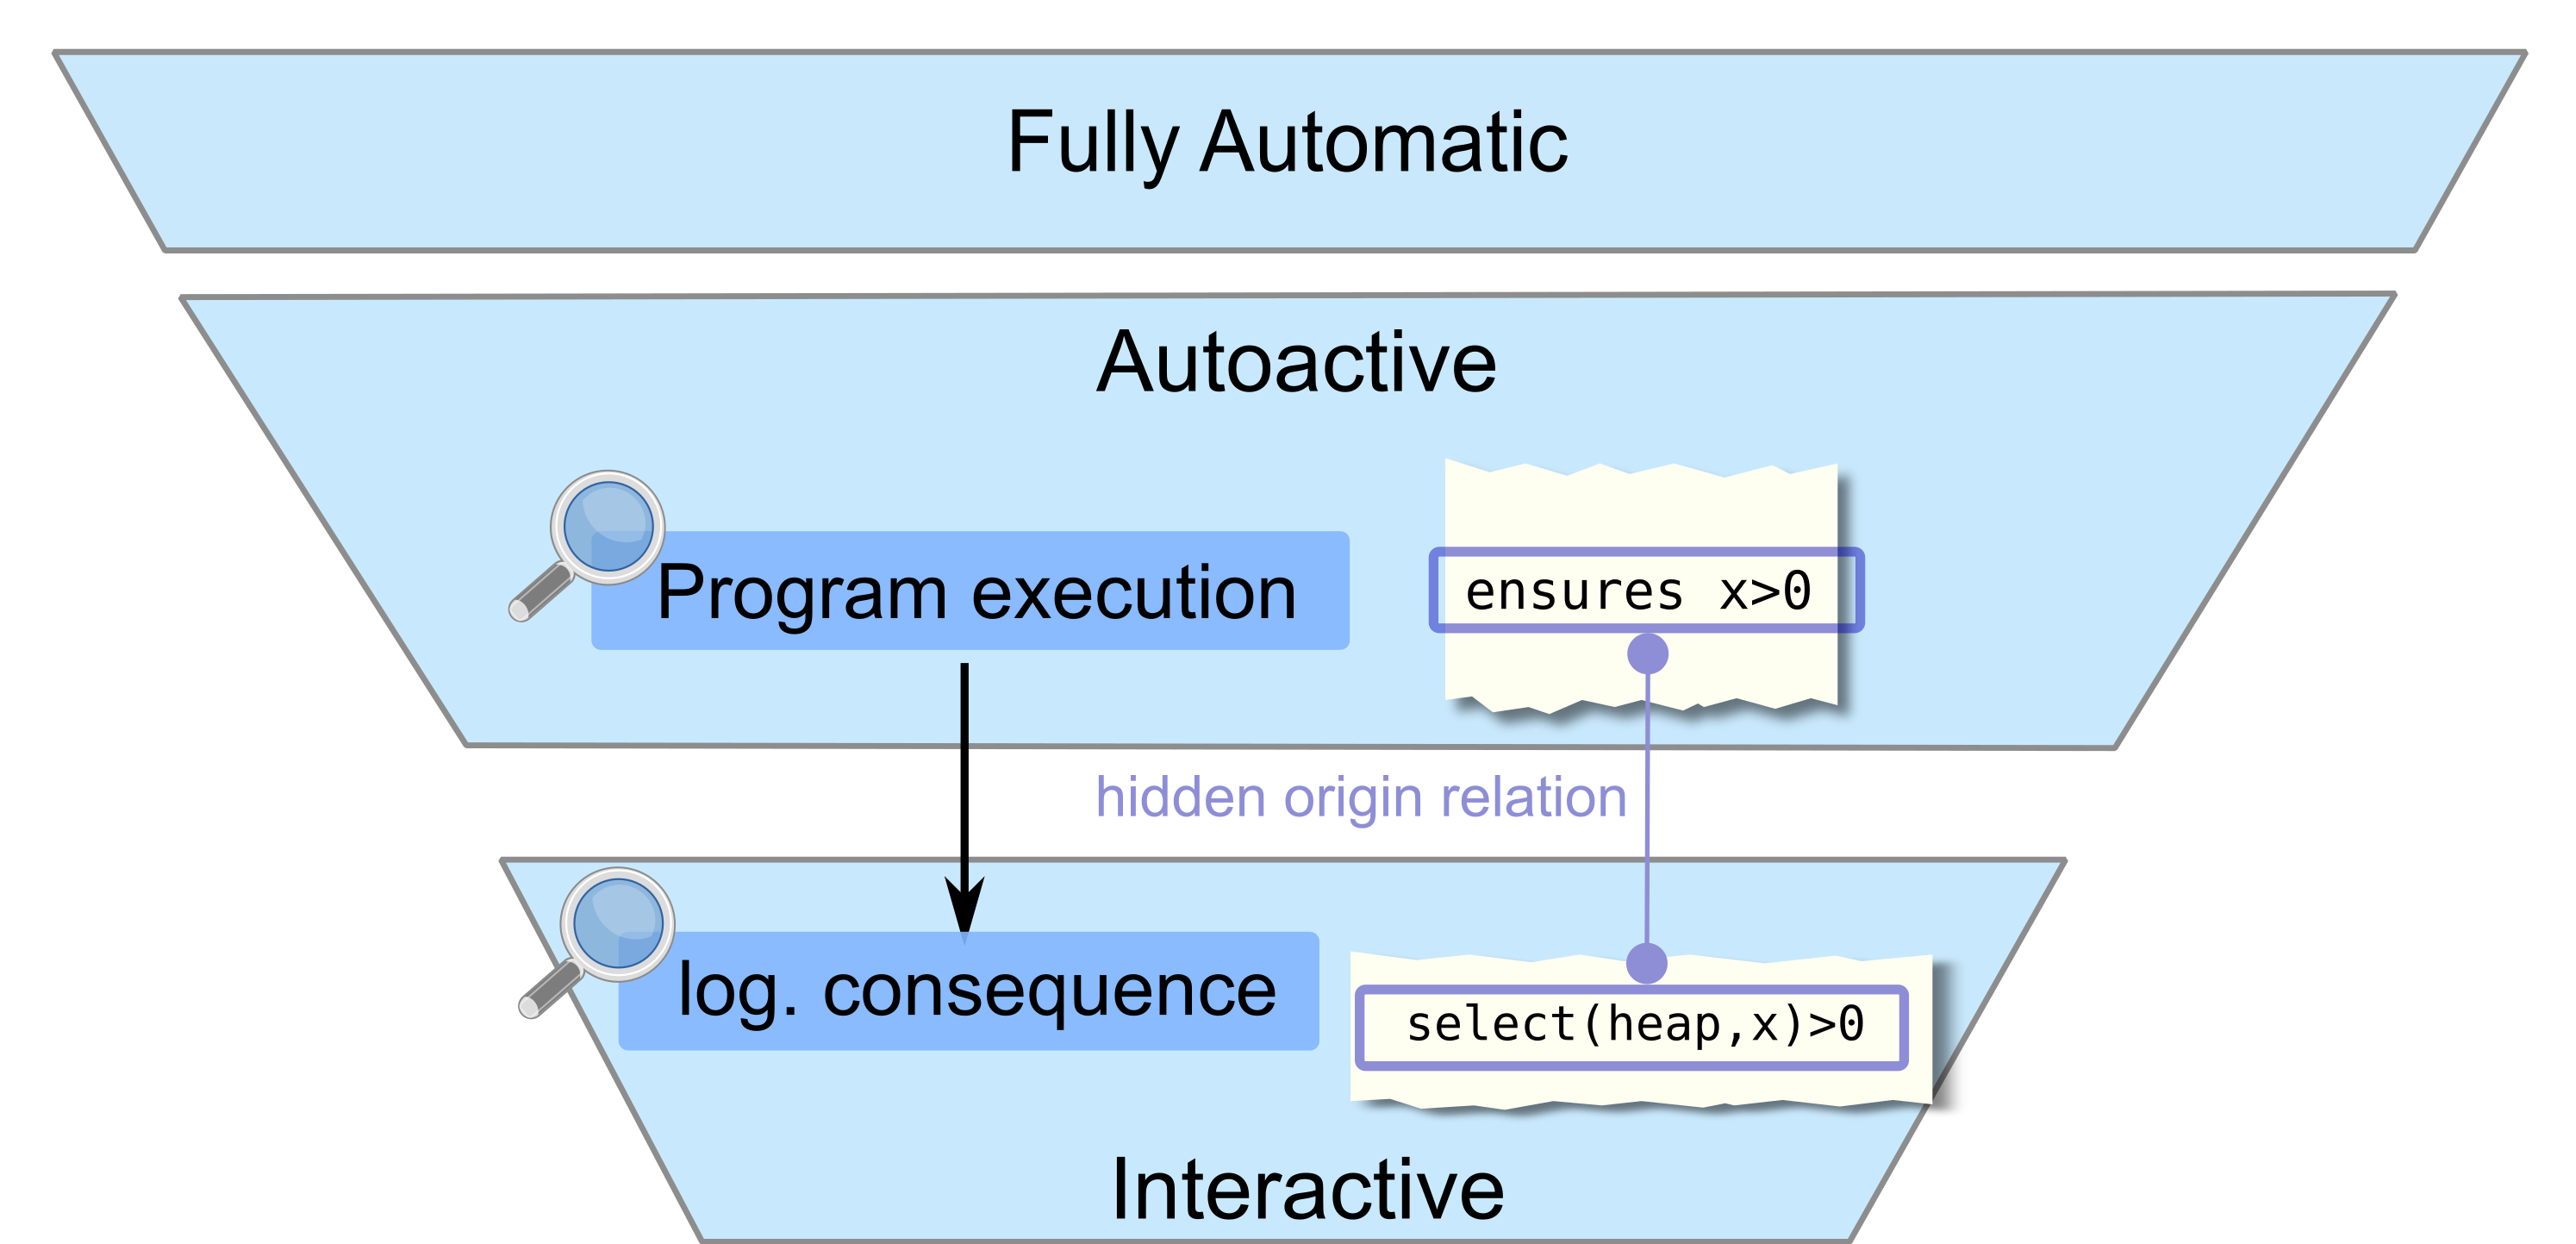
\includegraphics[width=\textwidth]{ipv3.png}}
\only<4> { 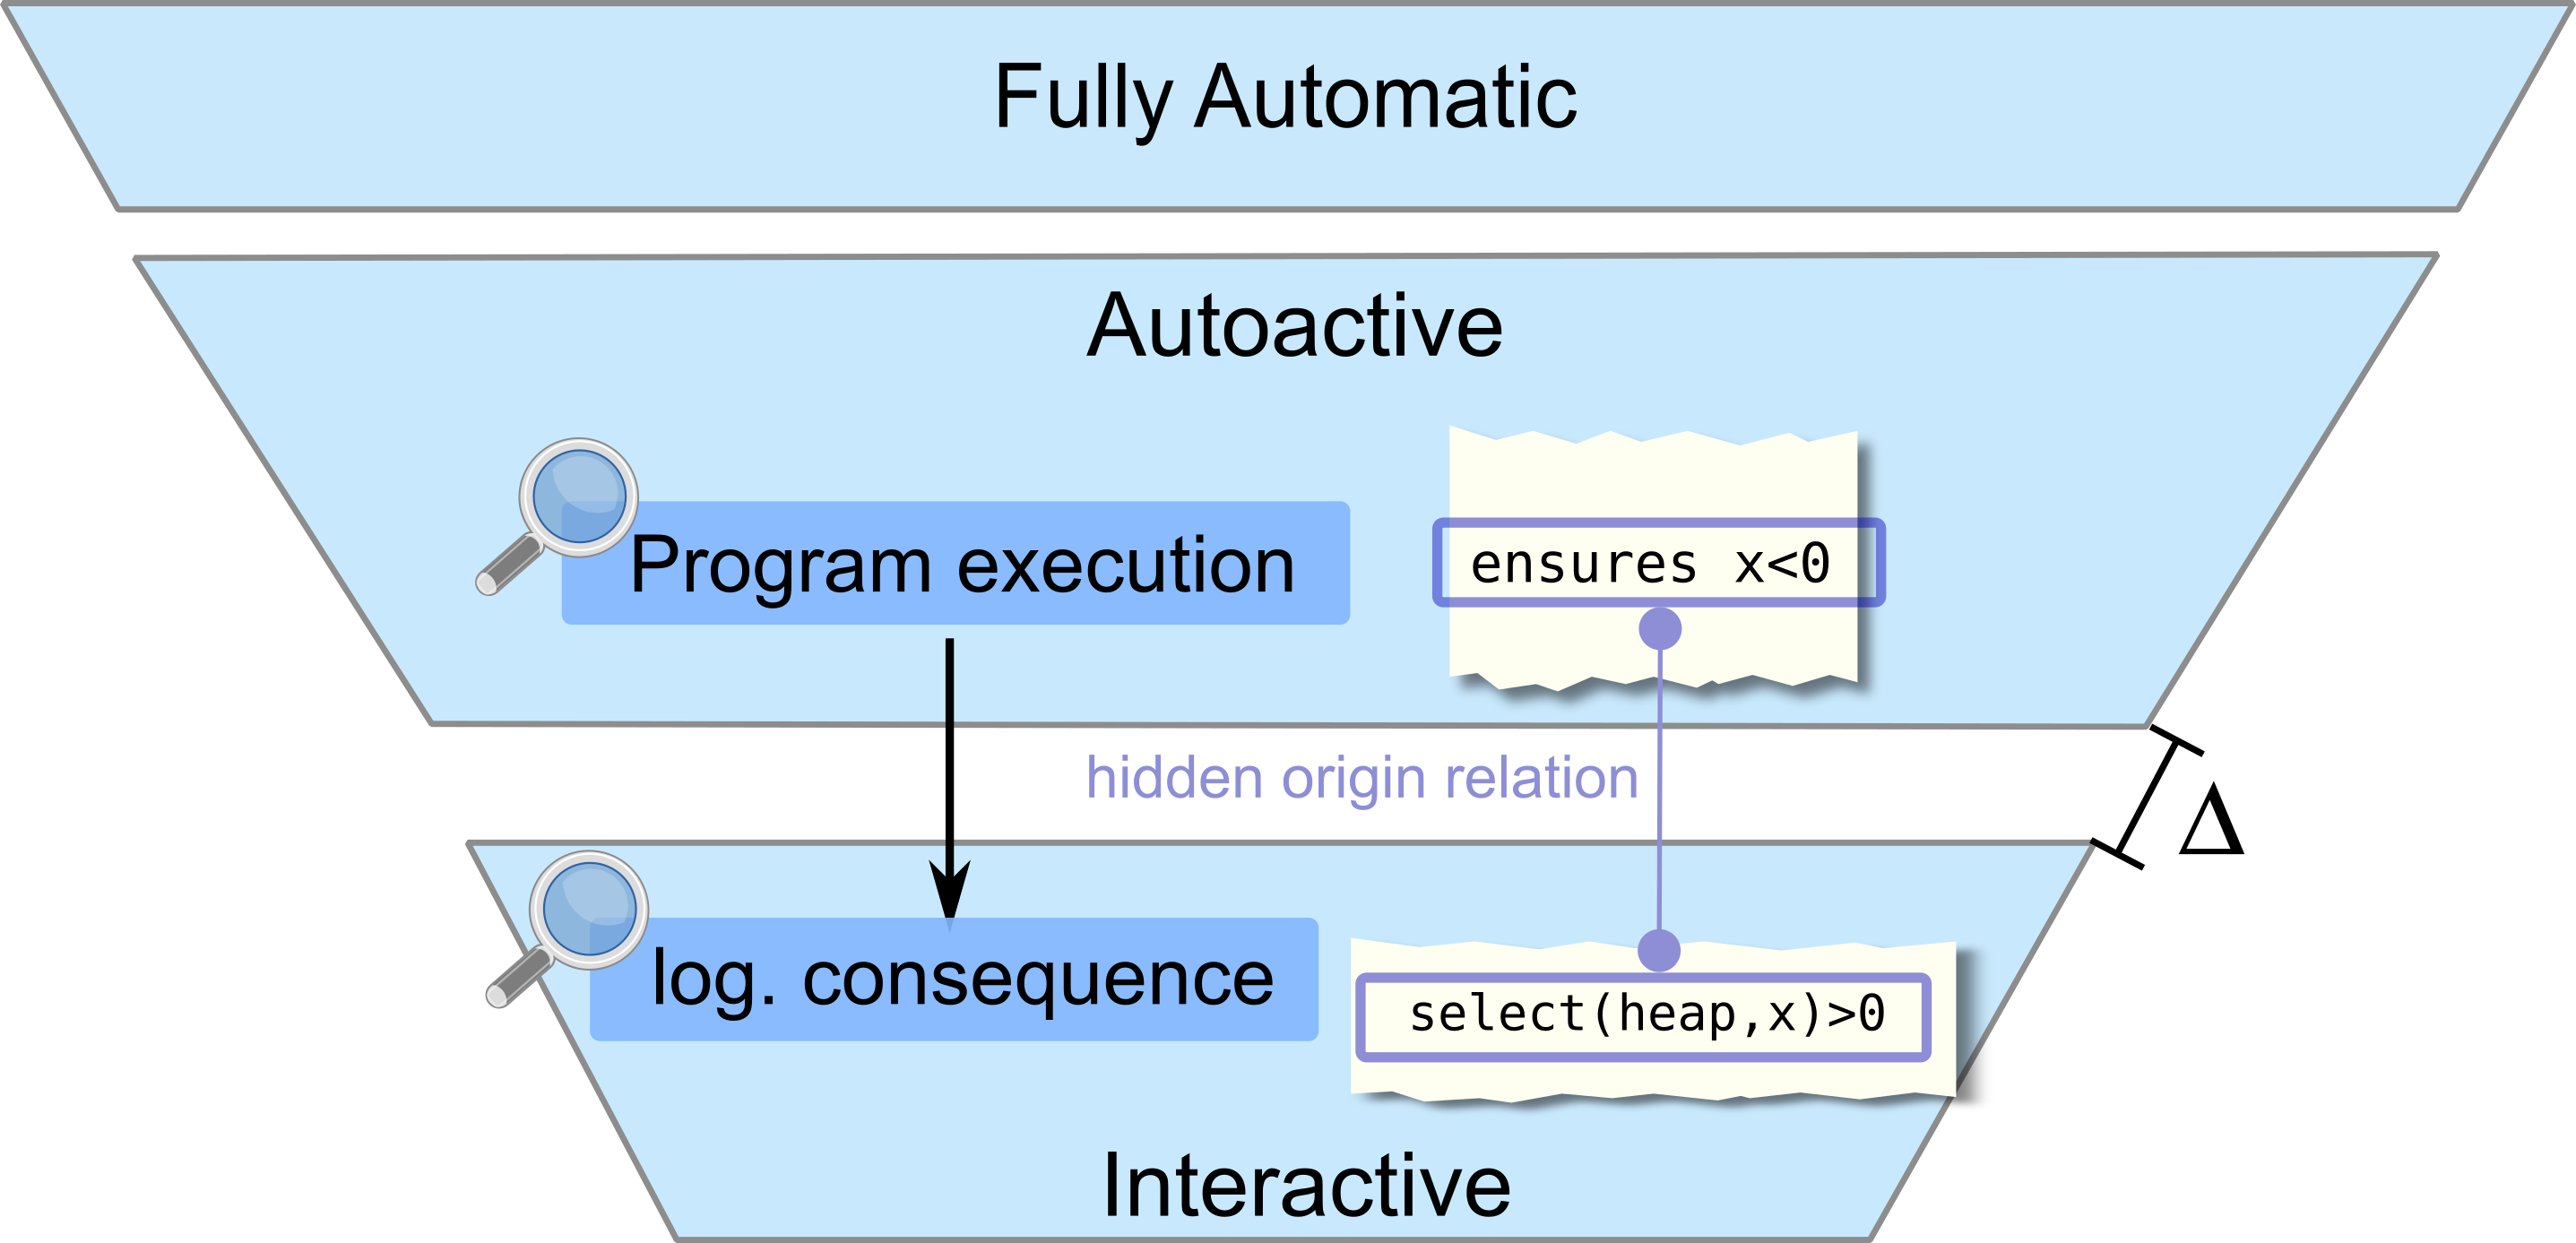
\includegraphics[width=\textwidth]{ipv4.png}}

% 	\begin{itemize}
% 		%\item Program Verification $\equiv$ Verification of Code
% 		\item Proofs conducted on different levels
% 			\begin{itemize}
% 				\item the code itself (needs insight if not closing)
% 				\item the logic level (needs relation back to original program)
% 			\end{itemize}
% 		\item state of the art user interfaces focus only on one level, supporting features for other levels often insufficient 
% 		\item may hinder users from using/understanding it
% 	\end{itemize}
\end{frame}

%\begin{frame}[c]{Objectives}
%The user is ...
%\begin{enumerate}
%\item ... able to use an appropriate view at all times
%\item ... can easily switch views without loosing focus
%\item ... is able to understand the relation of views
%\item ... is able to determine the results of costly actions before applying them
%\end{enumerate}
%\end{frame}

\begin{frame}[c]{AlgoVer: Seamless Program Verification}
\begin{itemize}
 \item Interactive program verification for Dafny
 \begin{itemize}
 \item Symbolic execution (� la \KeY{})
 \item Innovative interaction concepts
 \item Calling z3
   \end{itemize}

 \item Bridging the gap between code and proof
\end{itemize}

% 	\begin{itemize}
% 		\item allows to inspect different parts of the proof in individual views		
% 		\item supports insight into unfinished proof attempts
% 		\item seamless transition between different views
% 		\item conduction proofs possible via
% 		\begin{itemize}
% 			\item direct manipulation
% 			\item script based
% 			\item annotation based
% 		\end{itemize}
% 	\end{itemize}
\end{frame}

\begin{frame}{Demo}
\begin{center}
\Huge{Demo} 
\end{center}
\end{frame}

\begin{frame}{Features And Future Work}
Features:
	\begin{itemize}
		\item Inspection of different parts of the proof in individual views		
% 		\item supports insight into unfinished proof attempts
		\item Seamless transition between different views
		\item Proof construction using
		\begin{itemize}
			\item direct manipulation
			\item script based
			\item annotation based
		\end{itemize}
	\end{itemize}
\hspace{1em}

Future Work:
	\begin{itemize}
		\item More rules and strategies
		\item Improved SMT-support
		\item Feedback/Interaction back to annotations in source code
		\item Evaluation on larger examples
		\item ...
	\end{itemize}
\end{frame}

\end{document}
